\subsection{Detector overview}

ATLAS (A Toroidal LHC ApparatuS) is the largest volume detector ever constructed for a particle collider.
It has the dimensions of a cylinder with 46 meters long, 25 meters in diameter, and sits in a cavern 100 meters below ground.
The detector contains about 3000km of cables and it weights 7000 tonnes.

This paragraph briefly summarizes the coordinate system and nomenclature used to describe the ATLAS detector \cite{Collaboration_2008}.
As shown in figure~\ref{fig:coordinate}, we define the nominal interaction point as the origin of the coordinate system, the beam direction as the \textit{z}-axis and the \textit{x-y} plane is transverse to the beam direction.
The positive \textit{x}-axis is defined to be the direction pointing to the center of the LHC ring, 
while the positive \textit{y}-axis is pointing upwards.
\begin{figure}[!htb]
  \centering
  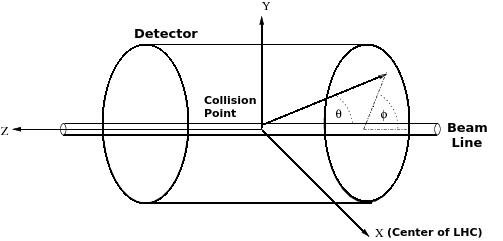
\includegraphics[width=0.9\textwidth]{figures/Detector/Coordinate_system_atlas.png}
  \caption{Coordinate system used by the ATLAS experiment at the LHC \cite{Perez:phdthesis}.}
  \label{fig:coordinate}
\end{figure}
There are two sides of detector A and C, in which A(C)-side is defined as with positive (negative) \textit{z}.
The azimuthal angle $\phi$ is measured as usual around the beam axis, while the polar angle $\theta$ is the angle from the beam axis
In physics analysis, we usually use the pseudorapidity instead of $\theta$ angle, which is designed as $\eta = - ln [tan\left( \frac{\theta}{2}\right)]$. 
For massive objects (eg. jets), the rapidity $y = \frac{1}{2} ln[ \frac{E+p_{z}}{E-p_{z}}]$ is used.
In addition, the \textit{transverse} momentum $p_{T}$, \textit{transverse} energy $E_{T}$ and the missing \textit{transverse} energy $E_{T}^{miss}$ are defined in \textit{x-y} plane.
The commonly used distance measurement $\Delta R$, is defined in the pseudorapidity-azimuthal angle space as $\Delta R = \sqrt{ \Delta\eta^{2} + \Delta\phi^{2}}$.

The overall ATLAS layout is shown in figure~\ref{fig:atlas_layout}, which is forward-backward symmetric with respect to the interaction point.
\begin{figure}[!htb]
  \centering
  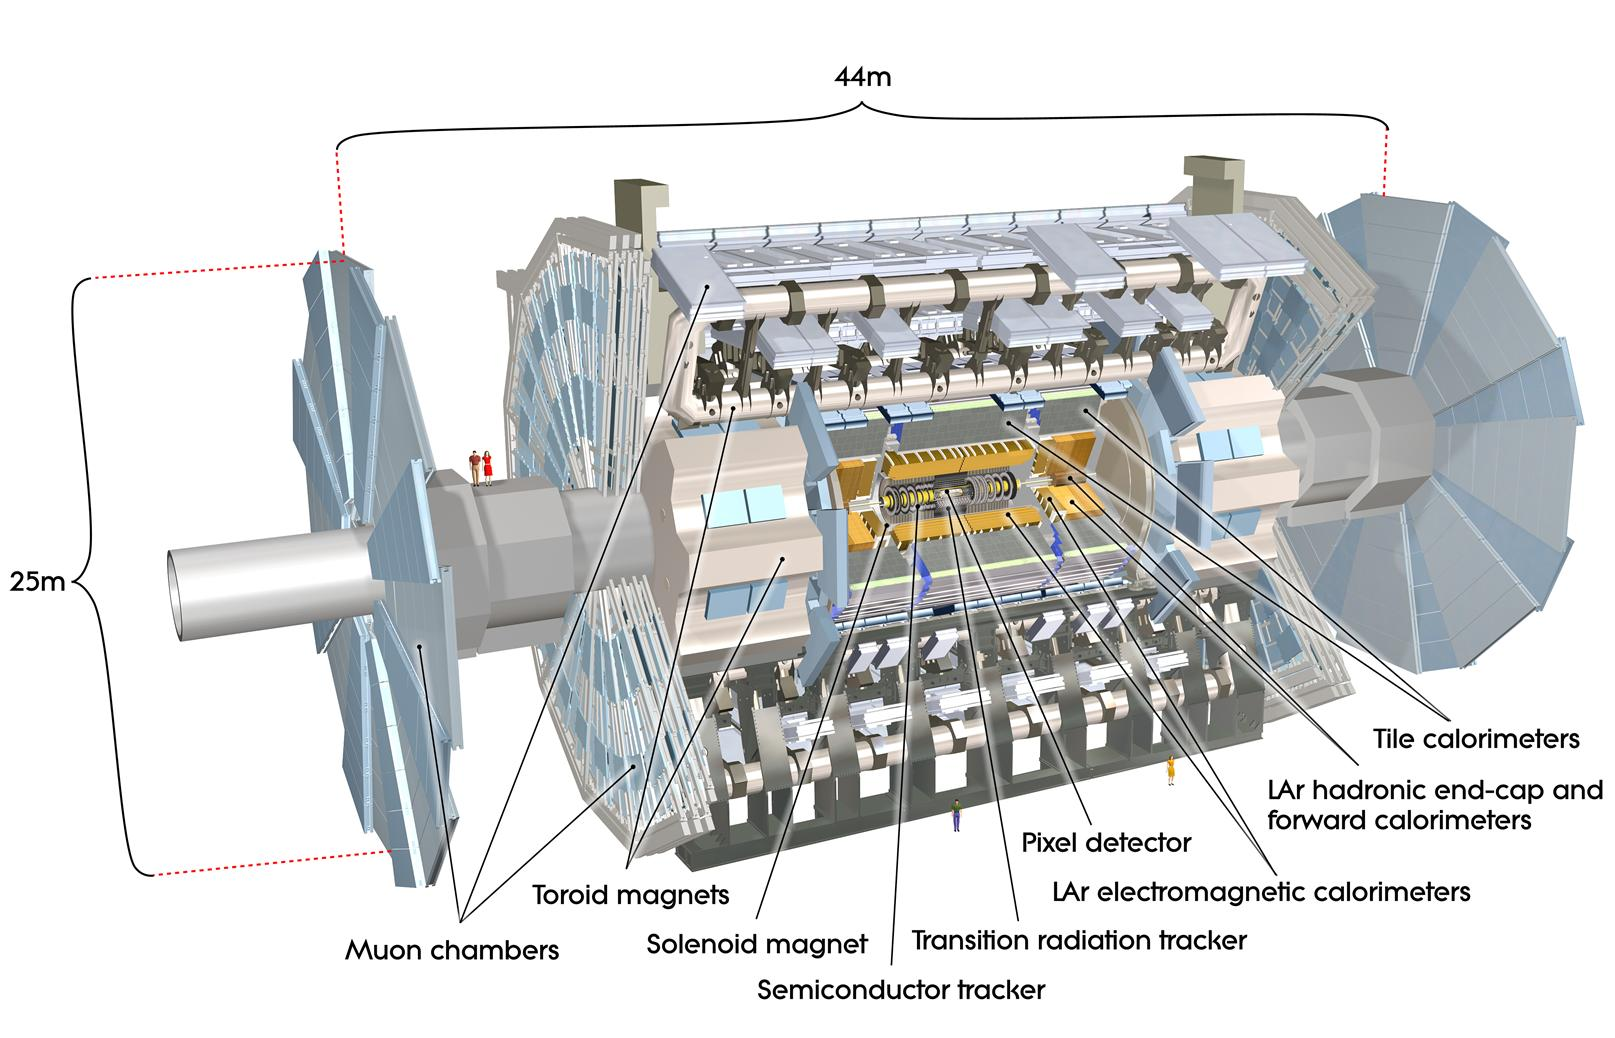
\includegraphics[width=1.0\textwidth]{figures/Detector/atlas_layout.jpg}
  \caption{Cut-away view of the ATLAS detector \cite{Pequenao:1095924}.}
  \label{fig:atlas_layout}
\end{figure}
The magnet configuration comprises a thin superconducting solenoid surrounding the inner-detector cavity, 
and three large superconducting toroids (one barrel and two end-caps) arranged with an eight-fold azimuthal symmetry around the calorimeters.

\textbf{The inner detector}, which is the innermost part of ATLAS, is immersed in a 2 T solenoidal magnetic field.
It's used for pattern recognition, momentum and vertex measurements and electron identification, with the combination of tracking system.

\textbf{The calorimeter} is outside the inner detector, for electromagnetic and hadronic energy measurements.
High granularity liquid-argon (LAr) electromagnetic sampling calorimeters is used to measure energy and position resolution with range up to $|\eta| < 3.2$ for electrons and photons.
For hadronic calorimetry, a scintillator-tile calorimeter is used in the range of $|\eta| < 1.7$.
The LAr forward calorimeters provide both electromagnetic and hadronic energy measurements with the coverage up to $|\eta| = 4.9$.

\textbf{The muon spectrometer} is in the outermost side.
The air-core toroid system, with a long barrel and two inserted end-cap magnets, provides strong bending power in a large volume within a light and open structure.
Multiple-scattering effects are minor, and excellent muon momentum resolution can be achieved.
